\documentclass[a4paper,12pt,openany]{memoir}
\usepackage[utf8]{inputenc}
\usepackage[russian]{babel}
\usepackage{indentfirst,amsmath,graphicx,pgf}

% Настройка: размер текста
\settypeblocksize{250mm}{160mm}{*}
\setulmargins{*}{*}{1}
\setlrmargins{*}{*}{1}
\checkandfixthelayout

% В русскоязычных книгах и статьях знаки равенства/неравенства, сложения,
% вычитания и умножения принято в случае переноса формулы на другую строку
% дублировать
\renewcommand\ne{\mathchar"3236\mathchar"303D\nobreak
      \discretionary{}{\usefont
      {OMS}{cmsy}{m}{n}\char"36\usefont
      {OT1}{cmr}{m}{n}\char"3D}{}}
\begingroup
\catcode`\+\active\gdef+{\mathchar8235\nobreak\discretionary{}%
 {\usefont{OT1}{cmr}{m}{n}\char43}{}}
\catcode`\-\active\gdef-{\mathchar8704\nobreak\discretionary{}%
 {\usefont{OMS}{cmsy}{m}{n}\char0}{}}
\catcode`\=\active\gdef={\mathchar12349\nobreak\discretionary{}%
 {\usefont{OT1}{cmr}{m}{n}\char61}{}}
\endgroup
\def\cdot{\mathchar8705\nobreak\discretionary{}%
 {\usefont{OMS}{cmsy}{m}{n}\char1}{}}
\def\times{\mathchar8706\nobreak\discretionary{}%
 {\usefont{OMS}{cmsy}{m}{n}\char2}{}}
\def\approx{\mathchar12825\nobreak\discretionary{}%
 {\usefont{OMS}{cmsy}{m}{n}\char25}{}}
\AtBeginDocument{%
\mathcode`\==32768%
\mathcode`\+=32768%
\mathcode`\-=32768%
}

% Для переносов слов с дефисами
\lccode`\-=`\-\defaulthyphenchar=127

% Намного лучше, чем \sloppy
\emergencystretch=2pt
\hfuzz=0.8pt

% Устраняем большие расстояния (по вертикали) в списках
\tightlists

% Для русского языка разделителем в подписях рисунков и таблиц служит точка
\captiondelim{.\space}
% Используем уменьшенный шрифт для подписей
\captionnamefont{\small}
% Величина пробела до и после рисунков и таблиц 
\setlength{\intextsep}{10pt}
% Нумерация рисунков и таблиц сплошная по всему документу
\renewcommand{\thefigure}{\arabic{figure}}
\renewcommand{\thetable}{\arabic{table}}

% Оформление списка литературы
\setbiblabel{[#1]\hfill}
\renewcommand{\bibsection}{%
  \section*{Список литературы и интернет-ресурсов}
  \prebibhook}
\newcommand{\link}[1]{\texttt{#1}}

% Оформление секций
\makeatletter
\renewcommand*{\thesection}{\@arabic\c@section.}
\setsecnumformat{\csname the#1\endcsname\space}
\makeatother

% Оформление страниц -- простейшее (с нумерацией внизу)
\pagestyle{plain}

\begin{document}
\thispagestyle{empty}

\vspace*{-\headheight}\vspace*{-\headsep}

{\centering\textsc{ 
министерство образования и науки РФ\\
московский государственный индустриальный университет\\
кафедра информационных систем и технологий\\
}

\vspace{4cm plus 1mm minus 1mm}

\begin{flushright}
\begin{tabular}{l}
Руководители работы:\\
доцент, к.т.н. Куприянов Д.Ю.\\
ассистент Александров А.И.
\end{tabular}
\end{flushright}

\vspace{3cm plus 1mm minus 1mm}

Войнов Максим Александрович

\vspace{1cm plus 1mm minus 1mm}
{\large\textbf{
<<Разработка Информационной системы учета успеваемости и посещаемости слушателей ФДО МГИУ>>
}}

\vspace{1cm plus 1mm minus 1mm}

Курсовая работа по дисциплине\\
<<Проектирование и разработка корпоративных информационных систем>>\\
4-й курс, 7-й семестр

\vfill

Москва 2011

}

\newpage
\endinput

% �������� ������� ���������� �����
\setcounter{page}{2}

\vspace*{1cm}
\section*{���������}
\begin{quote} 
�������� ������ ��������� ������������ ���������� ������� "��������", ����������� ���������� PostgreSQL. �������������� ��� ����������������� ������� �������� PostgreSQl.
{\em 

}
\end{quote}

\vspace*{1cm}

\tableofcontents

\endinput

\newpage
\section{Введение}
Последние пять лет ознаменовались фантастическим развитием Интернета и новых способов общения между людьми. На переднем крае этого явления находится \textit{World Wide Web (WWW)}. Ежедневно в этой новой коммуникационной среде открываются тысячи новых сайтов, а потребителям предлагаются новые виды услуг. Вместе с бурным развитием рынка появился огромный спрос на новые технологии и разработчиков, владеющих ими. Комплексная веб разработка сайтов различной тематики и направленности предусматривает создание нового или оптимизацию под нужные характеристики уже готового шаблона сайта, выбор и установку наиболее подходящей системы управления контентом и, при необходимости, заполнение ресурса контентом.Чтобы создать удобный и функциональный web-сайт используют различные технические средства, например HTML,  JavaSvript, Flash, различные СУБД. В данной работе были использованы HTML, СУБД PostgreSQL и платформа \textit{RubyOnRails}.\\

\hspace*{0.5cm}\textit{RubyOnRails} -- это полноценный, многоуровневый Фреймворк для построения веб-приложений, использующих базы данных, который основан на архитектуре Модель-Представление-Контроллер (Model-View-Controller, MVC). Динамичный \textit{AJAX} -- интерфейс, обработка запросов и выдача данных в контроллерах, предметная область, отраженная в базе данных, — для всего этого Rails предоставляет однородную среду разработки на Ruby.\\

\endinput


\newpage
\section{MVC}

\textbf{Model-view-controller} (MVC, «Модель - Представление - Контроллер») -- шаблон проектирования, в котором модель данных приложения, пользовательский интерфейс и управляющая логика разделены на три отдельных компонента так, что модификация одного из компонентов оказывает минимальное воздействие на остальные. Шаблон MVC позволяет разделить данные, представление и обработку действий пользователя на три отдельных компонента:

\begin{itemize}
\item Модель (Model). Модель предоставляет данные (обычно для View), а также реагирует на запросы (обычно от контроллера), изменяя своё состояние.
\item Представление (View). Отвечает за отображение информации (пользовательский интерфейс).
\item Поведение (Controller). Интерпретирует данные, введённые пользователем, и информирует модель и представление о необходимости соответствующей реакции.
\end{itemize}

Важно отметить, что как представление, так и поведение зависят от модели. Однако модель не зависит ни от представления, ни от поведения. Это одно из ключевых достоинств подобного разделения. Оно позволяет строить модель независимо от визуального представления, а также создавать несколько различных представлений для одной модели.

\endinput



\newpage
\section{Структура базового проекта}

\hspace*{0.5cm}Рассмотрим структуру базового проекта. Для этого воспользуемся диаграммой классов UML. Диаграммы классов используются при моделировании программных систем (ПС) наиболее часто. Они являются одной из форм статического описания системы с точки зрения ее проектирования, показывая ее структуру. Диаграмма классов не отображает динамическое поведение объектов изображенных на ней классов. На диаграмме классов показываются классы, интерфейсы и отношения между ними.
\begin{figure}[h!]
\begin{center}
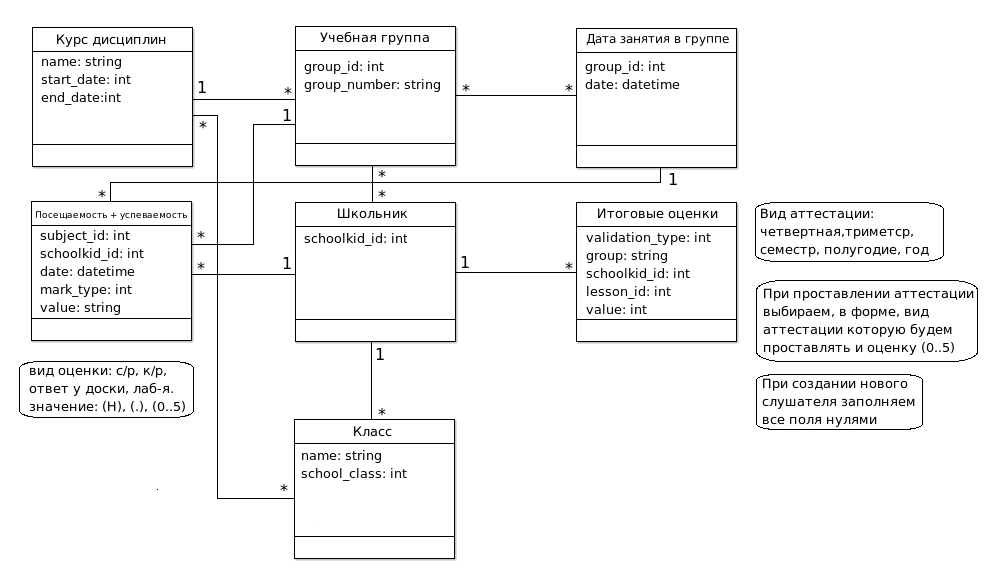
\includegraphics[scale=0.6]{image/class_my.png}
\end{center}
\caption{Диаграмма классов}
\end{figure}
\hspace*{0.5cm}Из данной диаграммы видно, что в системе присутствуют такие классы как:\\
\begin{itemize}
\item курс дисциплин;
\item учебная группа;
\item школьник;
\item посещаемость и успеваемость;
\item дата занятия в группе;
\item класс;
\item итоговые оценки;
\end{itemize}
\hspace*{0.5cm}Класс \textbf{Итоговые оценки} и класс \textbf{Посещаемость и успеваемость} -- классы хранилища, которые содержат информацию об успеваемости и посещаемости слушателей ФДО: оценки, информацию о посещаемости, и т.д. Класс \textbf{Итоговые оценки} находится в отношении один ко многим с классом \textbf{Школьник}.А класс \textbf{Посещаемость и успеваемость} связан отношением один ко многим, с классами \textbf{Школьник}, \textbf{Учебная группа} и \textbf{Дата занятия в группе}. Он содержит информацию о посещаемости и успеваемости слушателя ФДО на данный момент: Оценки и количество посещенных или пропущенных занятий.\\

\section{Разработанные модели}
\hspace*{0.5cm}Для начала определим, какие классы необходимо добавить в систему. Это будут следующие классы:\\
\begin{itemize}
\item \textbf{Школьники} - в этом классе будет храниться информация о школьниках. В этом классе следующие атрибуты: first\_name, second\_name, last\_name, birthday, male, addres, telephone, school\_group\_id, group\_id, created\_at, updated\_at.\\
\item \textbf{Дисциплины} - в данном классе хранится список существующих дисциплин, со следующими атрибутами: full\_name, short\_name, created\_at, updated\_at.\\
\item \textbf{Курсы} - содержит информацию о датах проведения курсов у слушателей ФДО. Имеет следующие атрибуты: start\_date, finish\_date, discipline\_id, created\_at, updated\_at.\\
\item \textbf{Школы} - хранится список школ, из которых поступают абитуриенты. Атрибуты : number, director\_name, director\_surname, director\_pathname, created\_at, updated\_at.\\
\item \textbf{Классы} - данный класс хранит информацию о школьных классах, в которых проходят обучение абитуриенты. Атрибуты : schoolkid\_id, group\_id, created\_at, updated\_at.\\
\item \textbf{Учебные группы} - хранится информация об учебных группа ВУЗа. Данный класс содержит следующие атрибуты : number, year, school\_id, stype, created\_at, updated\_at.\\
\end{itemize}
\endinput

\newpage
\section{Постановка задачи}
Реализовать систему добавления альбомов фотографий персон и кадров из фильма.\\
\hspace*{0.25cm}С точки зрения конечного пользователя это означает, что в системе должен быть предусмотрен интерфейс для добавления фильму и актеру альбома с фотографиями, отдельный интерфейс для просмотра добавленных фотографий.


\section{Пример реализации одного из классов}

\subsection{Использование генератора scaffold}
\hspace*{0.25см}Теперь, после определения классов и их атрибутов, которые будут в нашей системе, можно переходить к реализации.\\
Так как для каждого класса необходимы модель, контроллер и представления воспользуемся генератором \textit{scaffold}, и сгенерируем все части с его помощью.
\verbatiminput{code/sc.txt}
Для корректной работы системы необходимо правильно выстроить отношения. Возьмем к примеру классы <<Дисциплина>> и класс <<Курс>>. Для того чтобы связать эти классы отношением один ко многим, внесем изменения в модели \textbf{Discipline} и \textbf{Cource}\\
\verbatiminput{code/discipline.txt}
\verbatiminput{code/course.txt}
Cвязь один ко многим с классом \textbf{Course} (belongs\_to \:discipline). Также добавлены ограничения: Дата начала и конца дисциплины, а также идентификатор должны быть не пустыми.\\
В модель \textbf{Course} вводим метод attr\_reader, передаем переменную \:discipline\_token, он делает эту переменную доступной вне этого класса. И метод \textbf{discipline\_token}, для того чтобы можно было использовать jquery плагин под названием token\_input, который позволяет выбирать множество пунктов из предопределенного листа, используя автоподстановку для поиска каждого из элементов.\\

\subsection{Контроллер и Представление}
Теперь, после внесения всех необходимых изменений в модели, можно переходить к контроллерам. Контроллер интерпретирует данные, введённые пользователем, и информирует модель и представление о необходимости соответствующей реакции.\\
\hspace*{0.25cm}Для того чтобы пользователь мог добавлять курсы, нужно создавать отдельный интерфейс. Для этого просто добавим ссылку на страничку создания курса.\\
Рассмотрим, как это будет выглядеть для класса \textbf{Course}.
\verbatiminput{code/form.txt}
Необходимо добавить небольшой скрипт, который будет посылать запрос в фоновом режиме к контролеру и ожидать результатов поиска. При этом контролер может извлекать данные из любого места, как, например, базы данных или жесткого диска. Но результаты поиска должны возвращаться  в формате \textit{JSON}.
\verbatiminput{code/js.txt}
Также необходимо добавить создание, отображение, редактирование, удаление, изменение и сохранение нового курса в контроллере курса.\\
\verbatiminput{code/update.txt} 
Если пользователь, при создании нового курса, не ввел никакой информации, то он не сохранится. Если не удалось сохранить курс (а это возможно только в одном случае -- данные, введенные пользователем,  не прошли проверку), делается возврат в форму, и отображается сообщение об ошибке пользователю.\\
Для отображения уже созданных курсов необходимо внести изменения в представления \textbf{Index} и \textbf{Show}
\verbatiminput{code/show.txt}
\textit{Представление Show}
\verbatiminput{code/index.txt}
\textit{Представление Index}\\
\textbf{Аналогичным образом реализуются остальные классы.}
\endinput


\newpage
\section{Приложение}
\vspace*{1cm}
\subsection{Пример работы}
\vspace*{1cm}
Приведем пример работы тех изменений, которые мы внесли в эталонный проект.\\
\begin{figure}[h!]
\begin{center}
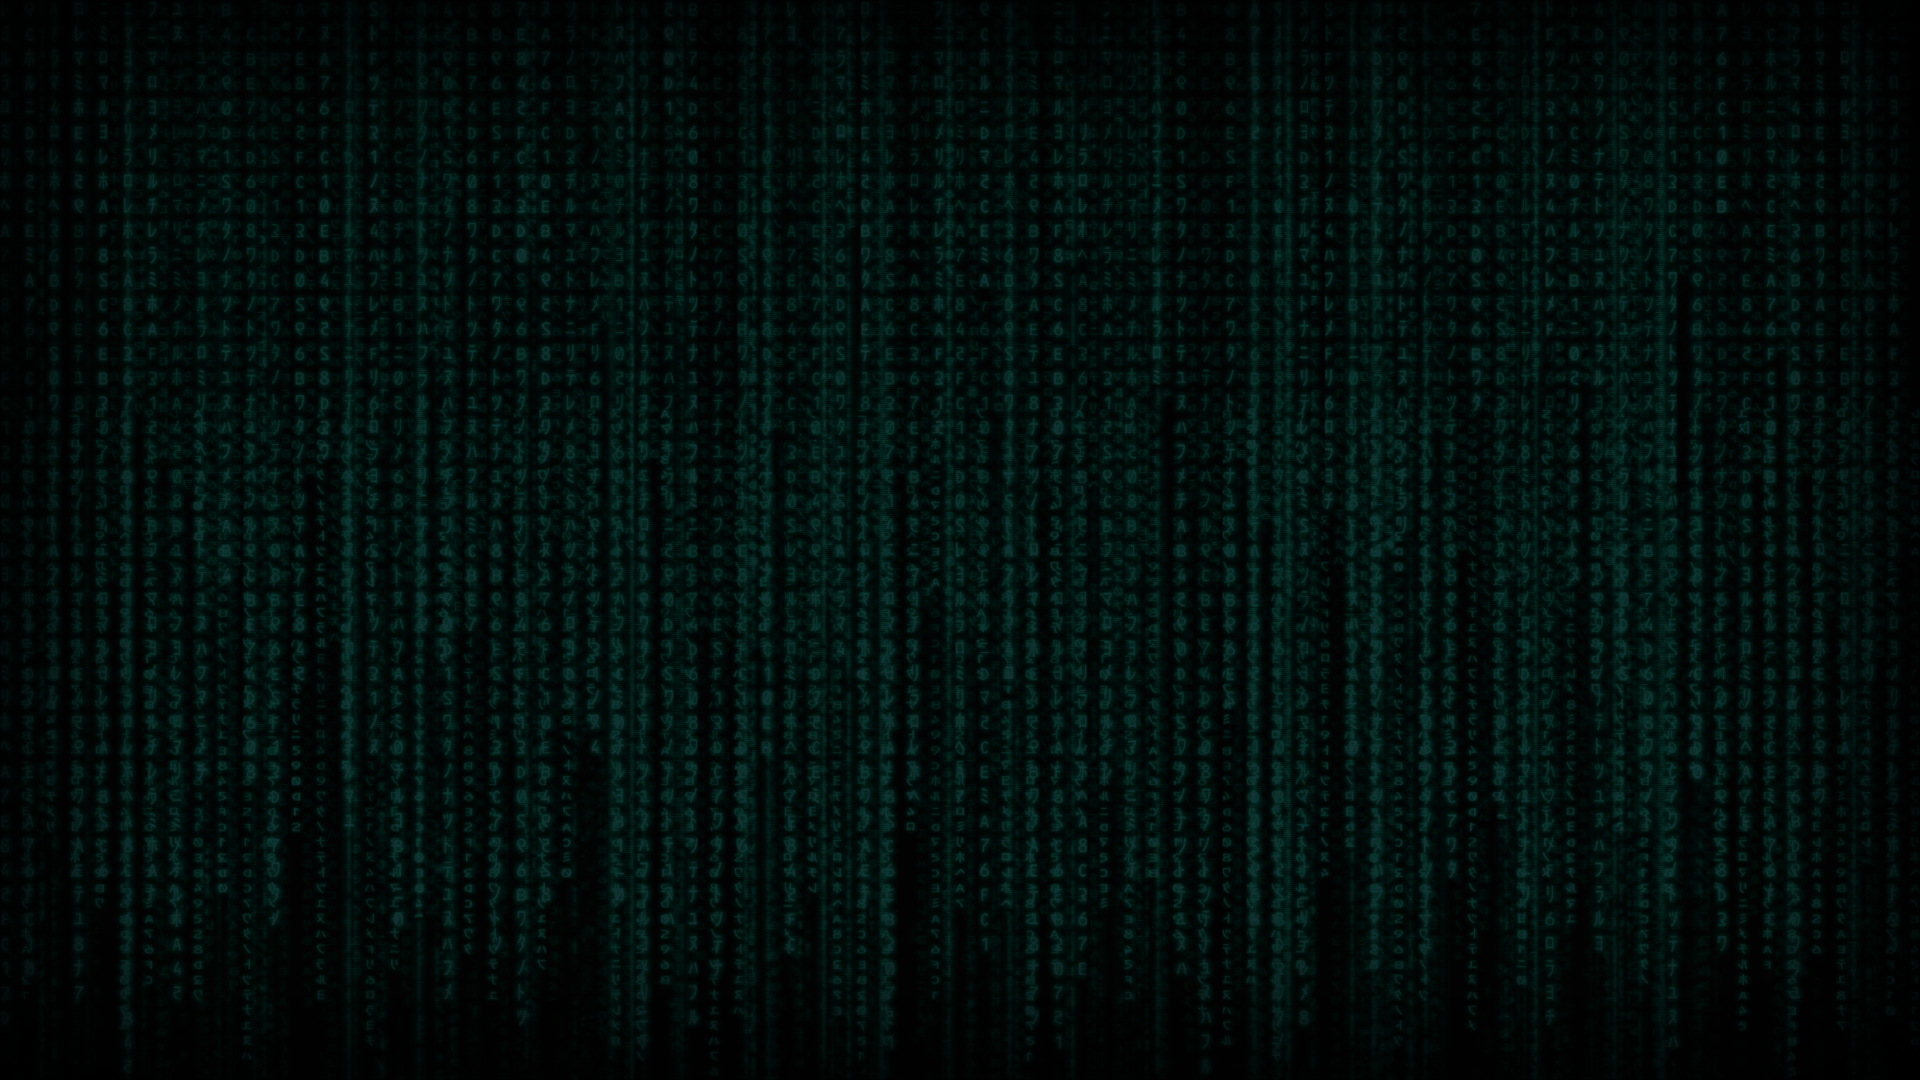
\includegraphics[scale=0.35]{image/1.png}
\end{center}
\newpage
\caption{Домашняя страничка}
\end{figure}
\newpage
Далее рассматривается, как будет выглядеть интерфейс просмотра альбома у конкретной персоны и фильма.\\
\begin{figure}[h!]
\begin{center}
\includegraphics[scale=0.25]{image/2.png}
\end{center}
\caption{Альбом у персоны}
\end{figure}
\begin{figure}[h!]
\begin{center}
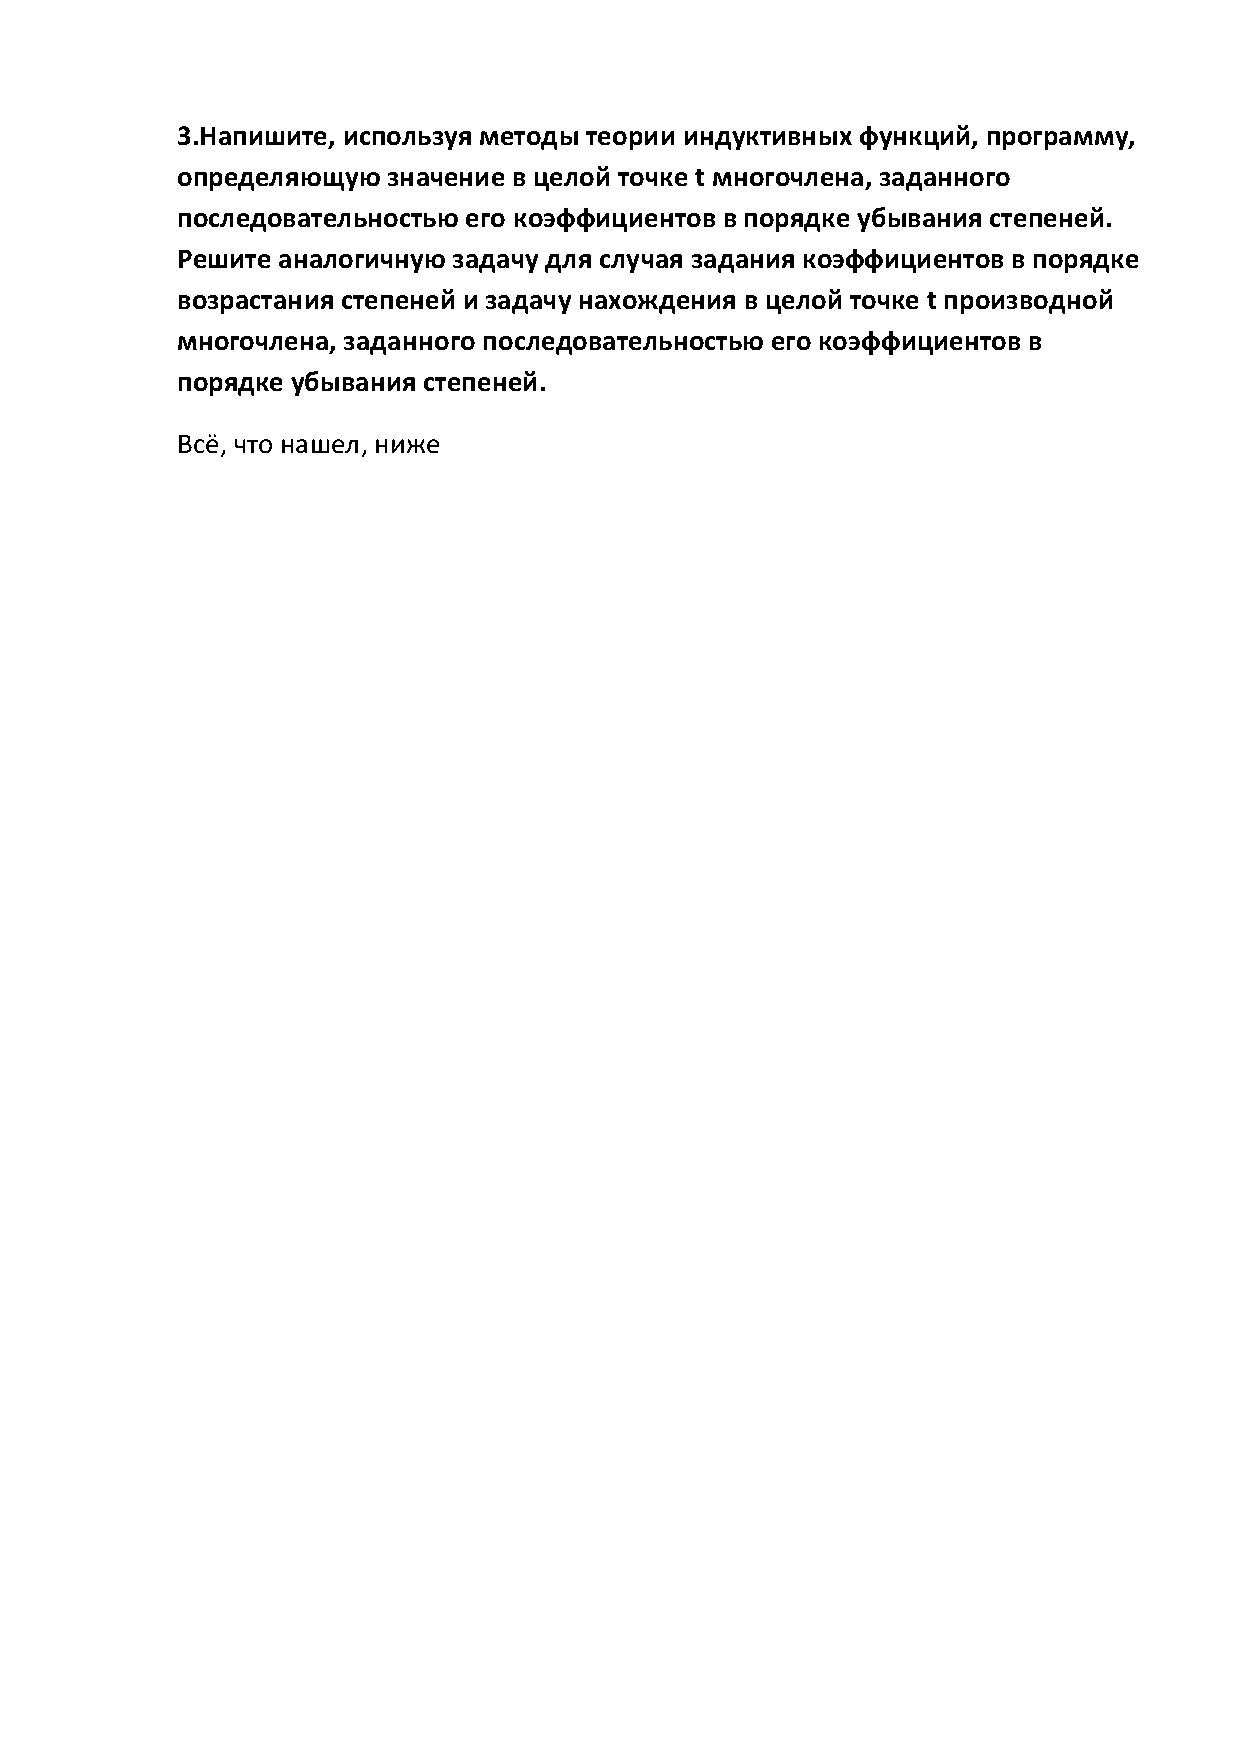
\includegraphics[scale=0.25]{image/3.png}
\end{center}
\caption{Альбом у фильма}
\end{figure}
\newpage
Для того чтобы добавить новый альбом, достаточно перейти по ссылке "Новый альбом". При нажатии произойдет перенаправление на страничку создания альбома.\\
\begin{figure}[h!]
\begin{center}
\includegraphics[scale=0.35]{image/4.png}
\end{center}
\caption{Добавление Альбома}
\end{figure}
\newpage
Если просто нажать кнопку "Сохранить" то отобразится сообщение об ошибке.\\
\begin{figure}[h!]
\begin{center}
\includegraphics[scale=0.35]{image/5.png}
\end{center}
\caption{Ошибка}
\end{figure}
Альбом должен быть закреплен, либо за персоной, либо за фильмом и никак иначе. Также продемонстрирован наглядный пример работы валидатора: название альбома должно существовать и должно содержать от 3 до 40 символов в названии
\newpage
\endinput

\newpage
\begin{thebibliography}{}

\bibitem{rlatex}
С.М. Львовский.
{\em Набор и вёрстка в системе \LaTeX, 3-е изд., испр. и доп.}~---
М., МЦНМО, 2003. Доступны исходные тексты этой книги.

\bibitem{wiki-LaTeX}
\link{http://ru.wikipedia.org/wiki/LaTeX}~---
Википедия (свободная энциклопедия) о системе \LaTeX.

\bibitem{sbras}
\link{http://www.sbras.ru/win/docs/TeX/LaTex2e/docs\_koi.html}~---
Различная документация по системе \LaTeX.

\bibitem{memoir}
\link{http://edgeguides.rubyonrails.org/}~---
Официальный сайт Ruby On Rails.

\bibitem{railscasts}
\link{http://railscasts.com/}
Видео уроки работы с Ruby On Rails.

\bibitem{apidoc}
\link{http://apidock.com/rails}
Электронная документация по Ruby On Rails 

\end{thebibliography}

\endinput

\end{document}

\endinput
